\chapter{Eksperymentalny algorytm klasyfikatora fingerprintów}

\section{Motywacja}
Wcześniej w niniejszej pracy zostało zaznaczone, że \emph{fingerprint} może być
bardziej unikalny kosztem jego stabilności i odwrotnie. Aby zgrupować kolejne
\emph{fingerprinty} tej samej przeglądarki internetowej, których różnice
wynikają z naturalnych przemian tej przeglądarki (np. aktualizacja), możemy użyć
klasyfikatora opartego na odpowiednim algorytmie. Tę relację przedstawia Rys. 7.
Dzięki takiemu rozwiązaniu jesteśmy w stanie zachować wiarygodny wskaźnik
entropii, używając średnio bardziej unikalnych \emph{fingerprintów} o mniejszej
stabilności.

Podobne (choć bardziej ograniczone) rozwiązanie zastosował Eckersley w swojej
pracy, w której po raz pierwszy opisał \emph{fingerprinting} przeglądarek
internetowych \cite[s. 13]{eckersley2010unique}.

\begin{figure}
	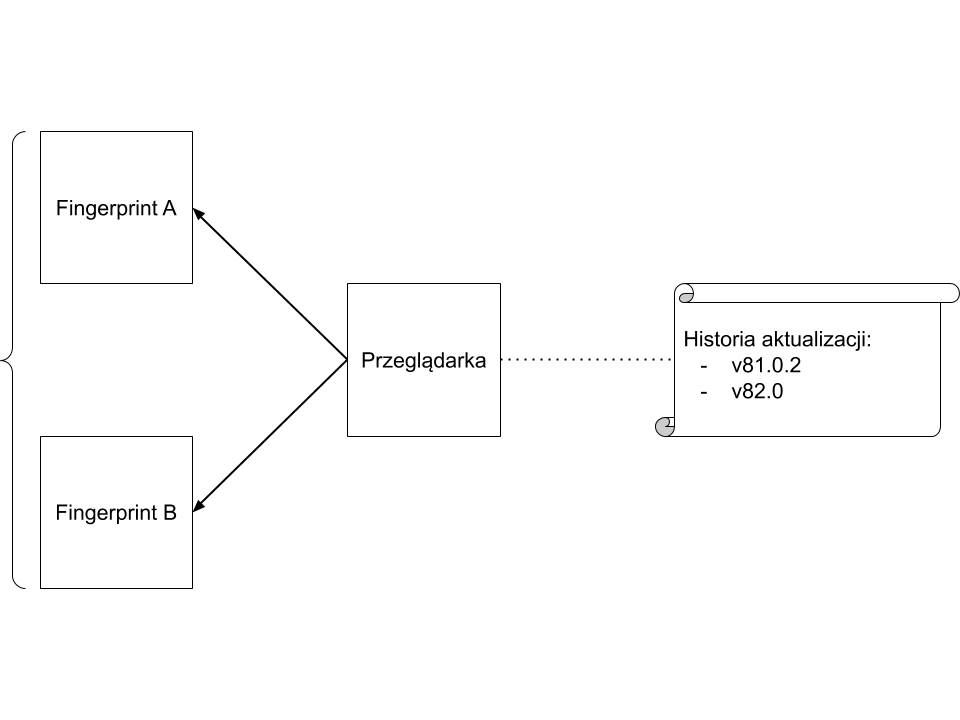
\includegraphics[width=\textwidth,keepaspectratio]{img/09}
	\source{Diagram przygotowany przez autora niniejszej pracy}
	\caption{Relacja \emph{fingerprint}--przeglądarka}
\end{figure}

\section{Opis algorytmu}
Aby zgrupować kolejne, podobne do siebie \emph{fingerprinty} należy wyznaczyć
podobieństwo każdego nowego \emph{fingerprintu} do wszystkich przechowywanych i
utożsamić go z tym, do którego jest najbardziej podobny (powyżej pewnej wartości
podobieństwa). Można to zrobić na parę sposobów. Jednym z najsensowniejszych
rozwiązań wydaje się podejście, w którym określa się podobieństwo cech
(komponentów) \emph{fingerprintu}, pomiędzy którymi istnieje relacja większości
(częściowy porządek). Tak można porównywać na przykład nagłówki User-Agent
(zawiera w sobie wersję oprogramowania) jako komponent dwóch porównywanych
\emph{fingerprintów}. Z tych porównań można wnioskować o ogólnym podobieństwie
dwóch \emph{fingerprintów}.

Porównywanie podobieństwa komponentów, które bezpośrednio lub pośrednio wynikają
z np. parametrów sprzętowych urządzenia (na przykład \emph{fingerprint} elementu
\texttt{canvas}), wydaje się bezcelowe. Ich wartość jest zwykle stała i
należałoby zastanowić się nad istnieniem częściowego porządku w takim zbiorze.
Jednakże ta niezmienność i dalej porównywanie tych komponentów na zasadzie
równoważności może być przydatne w szacowaniu, w jakim stopniu ogólne
podobieństwo jest wiarygodne.

Metryką określającą podobieństwo do siebie dwóch komponentów będzie odległość
Levenshteina, która jest powszechnie stosowaną miarą odmienności skończonych
ciągów znaków.

\subsection{Odległość Levenshteina}
Algorytmy wyznaczające odległość Levenshteina nie są na tyle popularne, aby
znalazły one swoją implementację w bibliotekach standardowych większości
popularnych języków oprogramowania. Z tego względu autor niniejszej pracy
zdecydował się na własnoręczną implementację.

\subsubsection{Definicja}
Odległość Levenshteina pomiędzy dwoma łańcuchami znaków \(a\) i \(b\) o
długościach odpowiednio \(i\) i \(j\), zdefiniowana jest jako
\begin{displaymath}
	\operatorname{ol}(i,j)=
	\begin{cases}
		\max(i,j)                    & \text{jeśli }\min(i,j)=0,  \\
		\min
		\begin{cases}
		\operatorname{ol}(i-1,j)+1 \\
		\operatorname{ol}(i,j-1)+1 \\
		\operatorname{ol}(i-1,j-1)   & \text{jeśli }a_i=b_j,      \\
		\operatorname{ol}(i-1,j-1)+1 & \text{jeśli }a_i \neq b_j. 
	\end{cases} & \text{w innym przypadku}.
	\end{cases}
\end{displaymath}

\subsubsection{Algorytm Wagnera--Fischera}
Bezpośrednia implementacja (z definicji) algorytmu wyznaczającego odległość
Levenshteina ma zasadniczy problem: tak zaimplementowany algorytm będzie działać
w czasie ponadwielomianowym. Aby się o tym przekonać, wystarczy narysować drzewo
wywołań rekurencyjnych i zauważyć, że kolejne wywołania nie są rozłączne (nie
jest to oczywiście formalny dowód). Wyznaczanie odległości Levenshteina cechuje
własność optymalnej podstruktury i bazując na programowaniu dynamicznym, można
znaleźć algorytm działający w czasie wielomianowym.

Jednym z takich algorytmów jest algorytm Wagnera--Fischera\footnote{Algorytm
	miał wielu wynalazców. Nazwa ,,Wagnera--Fischera'' powinna być traktowana
	jedynie jako zwyczajowa:
	https://en.wikipedia.org/wiki/Wagner-Fischer\_algorithm\#History} (Algorytm 2)
\cite{wagner1974string}. Implementacja 4 przedstawia implementację algorytmu
Wagnera--Fischera. Implementacja 5 jest optymalnym wariantem tego algorytmu
(biorąc pod uwagę zużycie pamięci; Implementacja 4 zużywa kwadratową ilość
pamięci a Implementacja 5 liniową). Taki wariant jest stosowany później w
algorytmie klasyfikatora.

\begin{algorithm}
	\SetAlgoVlined
	\SetAlgoCaptionSeparator{.}
	\SetKwInOut{Input}{Dane}
	\SetKwInOut{Output}{Wynik}
	\SetKwData{VarM}{m}
	\SetKwData{VarN}{n}
	\SetKwData{VarC}{c}
	\SetKwArray{VarA}{a}
	\SetKwArray{VarB}{b}
	\SetKwArray{VarD}{d}
	\SetKwArray{VarE}{}
	\SetKwFunction{Minimum}{minimum}
	\BlankLine
	\Input{ciągi znaków \VarA i \VarB o długościach odpowiednio \VarM i \VarN}
	\Output{odległość Levenshteina}
	\BlankLine
	\VarD $\leftarrow$ \VarE{$0 \dots$ \VarM, $0 \dots$ \VarN}\;
	\For{$i \leftarrow 1$ \KwTo \VarM}{
		\VarD{$i$, $0$} $\leftarrow i$\;
	}
	\For{$j \leftarrow 1$ \KwTo \VarN}{
		\VarD{$0$, $j$} $\leftarrow j$\;
	}
	\For{$j \leftarrow 1$ \KwTo \VarN}{
		\For{$i \leftarrow 1$ \KwTo \VarM}{
			\eIf{\VarA{$i - 1$} $=$ \VarB{$j - 1$}}{
				\VarC $\leftarrow 0$\;
				}{
				\VarC $\leftarrow 1$\;
			}
			\VarD{$i$, $j$} $\leftarrow$ \Minimum{\VarD{$i - 1$, $j$} $+$ $1$, \VarD{$i$, $j - 1$} $+$ $1$, \VarD{$i - 1$, $j - 1$} $+$ \VarC}\;
		}
	}
	\Return{\VarD{\VarM, \VarN}}\;
	\caption{Algorytm Wagnera--Fischera}
\end{algorithm}

\lstinputlisting[float,language=Go,caption=Algorytm Wagnera--Fischera w Go,firstline=18,lastline=44,tabsize=4]{go/levenshtein.go}

\lstinputlisting[float,language=Go,caption=Algorytm Wagnera--Fischera w Go (liniowa pamięć),firstline=46,lastline=74,tabsize=4]{go/levenshtein.go}

\section{Pseudokod}
Algorytm 3 obrazuje eksperymentalny algorytm klasyfikatora \emph{fingerprintów}.
Funkcja \texttt{hardwareRelatedCompatibility} odpowiada za binarne porównanie
wcześniej omawianych, teoretycznie niezmiennych komponentów. Funkcja
\texttt{similarity} bazując na odległości Levenshteina, przeprowadza porównanie
dla reszty komponentów. Implementacja 6 przedstawia implementację tego algorytmu
w Go.

% [ ] osCpu: getOsCpu
% [ ] languages: getLanguages
% [ ] colorDepth: getColorDepth
% [ ] deviceMemory: getDeviceMemory
% [ ] screenResolution: getScreenResolution
% [ ] availableScreenResolution: getAvailableScreenResolution
% [ ] hardwareConcurrency: getHardwareConcurrency
% [x] timezoneOffset: getTimezoneOffset
% [x] timezone: getTimezone
% [ ] sessionStorage: getSessionStorage
% [ ] localStorage: getLocalStorage
% [ ] indexedDB: getIndexedDB
% [ ] openDatabase: getOpenDatabase
% [ ] cpuClass: getCpuClass
% [?] platform: getPlatform
% [x] plugins: getPlugins
% [ ] canvas: getCanvasFingerprint
% [ ] touchSupport: getTouchSupport
% [x] fonts: getFonts
% [ ] audio: getAudioFingerprint
% [ ] pluginsSupport: getPluginsSupport
% [x] productSub: getProductSub
% [ ] emptyEvalLength: getEmptyEvalLength
% [ ] errorFF: getErrorFF
% [x] vendor: getVendor
% [ ] chrome: getChrome
% [ ] cookiesEnabled: areCookiesEnabled

\begin{algorithm}
	\SetAlgoVlined
	\SetAlgoCaptionSeparator{.}
	\SetKwInOut{Input}{Dane}
	\SetKwInOut{Output}{Wynik}
	\SetKwData{VarF}{f}
	\SetKwData{VarG}{g}
	\SetKwData{VarMax}{max}
	\SetKwData{VarRatio}{ratio}
	\SetKwData{VarCandidate}{candidate}
	\SetKwData{SetG}{G}
	\SetKwFunction{HardwareRelatedCompatibility}{hardwareRelatedCompatibility}
	\SetKwFunction{Continue}{continue}
	\SetKwFunction{Similarity}{similarity}
	\SetKw{Null}{NULL}
	\BlankLine
	\Input{Zbiór \emph{fingerprintów} \SetG i \emph{fingerprint} \VarF}
	\Output{\emph{fingerprint}, do którego \VarF jest najbardziej podobny, jeśli istnieje}
	\BlankLine
	\VarMax $\leftarrow 0$\;
	\ForEach{\VarG $\in$ \SetG}{
		\If{\HardwareRelatedCompatibility{\VarF, \VarG} $< \alpha$}{
			\Continue\;
		}
		\BlankLine
		\VarRatio $\leftarrow$ \Similarity{\VarF, \VarG}\;
		\BlankLine
		\If{\VarRatio $>$ \VarMax}{
			\VarMax $\leftarrow$ \VarRatio\;
			\VarCandidate $\leftarrow$ \VarG\;
		}
	}
	\If{\VarMax $\ge \beta$}{
		\Return{\VarCandidate}\;
	}
	\Return{\Null}\;
	\caption{Eksperymentalny klasyfikator}
\end{algorithm}

\section{Ocena złożoności czasowej i pamięciowej}
Załóżmy, że \texttt{hardwareRelatedCompatibility} działa w czasie stałym.
Zgodnie z wcześniejszym ustaleniami \texttt{similarity} powinna działać w czasie
co najwyżej kwadratowym, proporcjonalnym do długości \emph{fingerprintu}
(algorytm Wagnera--Fischera działa w czasie \(\Theta(mn)\), gdzie \(m\) i \(n\)
to długości porównywanych ciągów). Warto jednak zauważyć, że długość
\emph{fingerprintu} jest stała. Proponowany algorytm przegląda wszystkie
zapisane wcześniej \emph{fingerprinty} i dla każdego obrotu wykonuje stałą
pracę. Możemy zatem stwierdzić, że proponowany algorytm działa w czasie
liniowym.

Mając na uwadze rozważania z poprzedniego akapitu, możemy także stwierdzić, że
pamięć używana przez proponowany algorytm jest stała.

\section{Ocena efektywności}
